\chapter{Methodology}

In our exploration of various object detection architectures, it became clear that single-stage detector models, while notable for their efficiency, did not 
meet the accuracy demands required for small object detection. Given the challenges associated with detecting smaller objects, we considered multi-stage models
as a more viable solution, because these models are known for their enhanced precision and adeptness at handling intricate detection tasks. Through our research, 
a potential model combination emerged as a great candidate. The Feature Pyramid Network family of models excels in multi-scale representation essential for 
resolving objects of varying sizes, while the Vision Transformers family provides an exceptional ability to grasp global contextual dependencies within images
through the attention modules. 

By integrating these models, as a backbone and a detector we found that we can leverage the complementary strengths of both frameworks, thus creating a 
robust multi-stage model specifically made to achieve the best possible results in small object detection.

\section{Architecture}

Choosing a multi-stage model for small object detection does not necessarily imply that the model will be heavy in terms of trainable parameters or challenging 
to train. Our approach strategically combines the two types of models in order to harness their individual strengths while maintaining manageable complexity 
and training efficiency. This integration ensures that our multi-stage detector not only achieves an elevated accuracy but also remains practical in terms of 
computational resources and training time, making it a viable solution for real-world applications where both performance and efficiency are critical.

In this section we are going to describe and explain the model we developed in detail with the aim of successfully tackling the Small Object Detection challenge. 
The model we created is named Extended Masked-Attention Mask Transformer, a name based on the models we decided to integrate being the Extended Feature Pyramid 
Network[] and the Masked-Attention Mask Transformer (MAMT)[].

A very interesting finding in the EFPN article is that over the past years, rapid development of deep learning has boosted the popularity of 
CNN-based detectors and the improved overall accuracy and efficiency. Unfortunately they still perform poorly when detecting small objects with a few pixels. 
Since CNN uses pooling layers repeatedly to extract advanced semantics, the pixels of small objects can be filtered out during the down-sampling process.

\newpage
Utilization of low-level features is one way to pick up information about small objects. The FPN is the first method to enhance features 
by fusing features from different levels and constructing feature pyramids, where upper feature maps are responsible for larger object detection, and lower 
feature maps are responsible for smaller object detection. Despite FPN's improvement multi-scale detection performance, the heuristic mapping mechanism 
between pyramid level and proposal size in FPN detectors may confuse small object detection, since small-sized objects must share the same feature map with 
medium-sized objects and some large-sized objects.

\begin{figure}[h!]
    \centering
    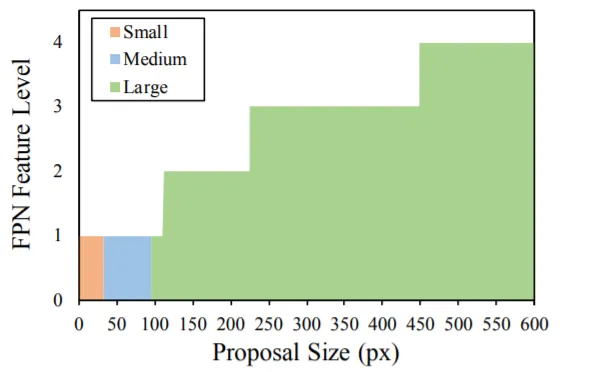
\includegraphics[scale=0.55]{Figures/efpn-sod-mapping.jpg}
    \caption{Small Object Detection Mapping}
    \label{fig:efpn-sod-mapping}
\end{figure}


\newpage
\subsection{Extended Feature Pyramid Network}

The implementation of the Extended Feature Pyramid follows closely an FPN-like framework embedded with a feature Super Resolution (SR)[] module. 
This pipeline directly generates high resolution features from low-resolution images to support small object detection, while stays in low computational 
cost. The top four pyramid layers are constructed by top-down pathways for medium and large object detection. 

The bottom extension of the EFPN  contains the very important FTT module, the top-down pathway and the purple pyramid layer in \ref{fig:efpn}, that aims to 
capture regional details for small objects. More specifically, in the extension, the third and fourth pyramid layers of EFPN which are denoted by green 
and yellow layers respectively in \ref{fig:efpn}, are mixed up in the feature super resolution module, the FTT with the aim of producing the intermediate 
feature $P'_{3}$ with selected regional information, which is denoted by a blue diamond in Figure \ref{fig:efpn}. Finally the top-down pathway merges $P'_{3}$ 
with a tailor-made high-resolution CNN feature map $C'2$, producing the final extended pyramid layer $P'2$.


\begin{figure}[h!]
    \centering
    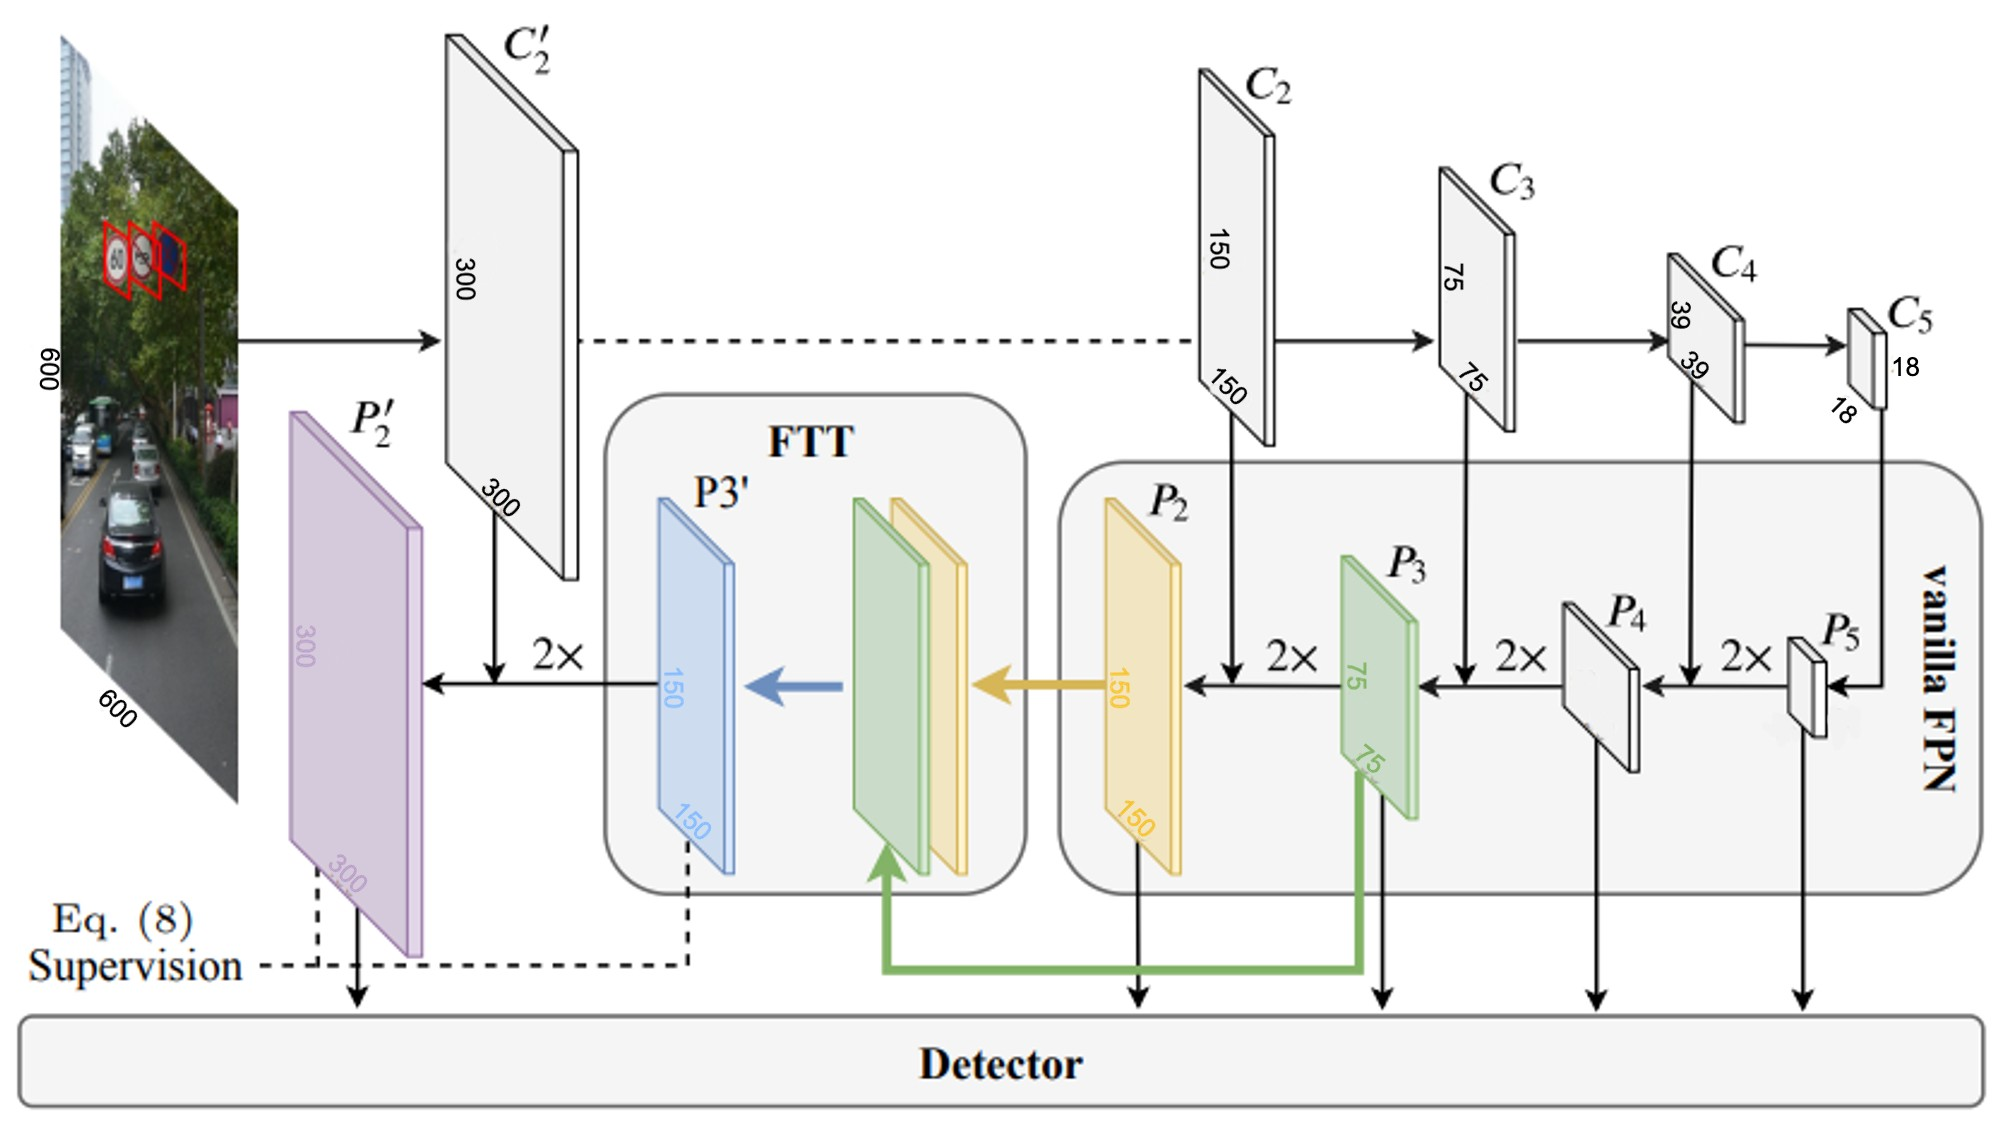
\includegraphics[scale=0.15]{Figures/efpn.jpg}
    \caption{Extended Feature Pyramid Network}
    \label{fig:efpn}
\end{figure}

The current Feature Texture Transfer (FTT) output as seen in the figure  synthesizes strong semantics in upper low-resolution features and critical local details in lower high-resolution 
reference features, but discards disturbing noises in reference. As shown in Figure \ref{fig:ftt}, the main input of FTT module is the feature map P3
from the 3rd layer of EFPN, and the reference is the feature map P2 from the 4th layer of EFPN. 

\begin{figure}
    \centering
    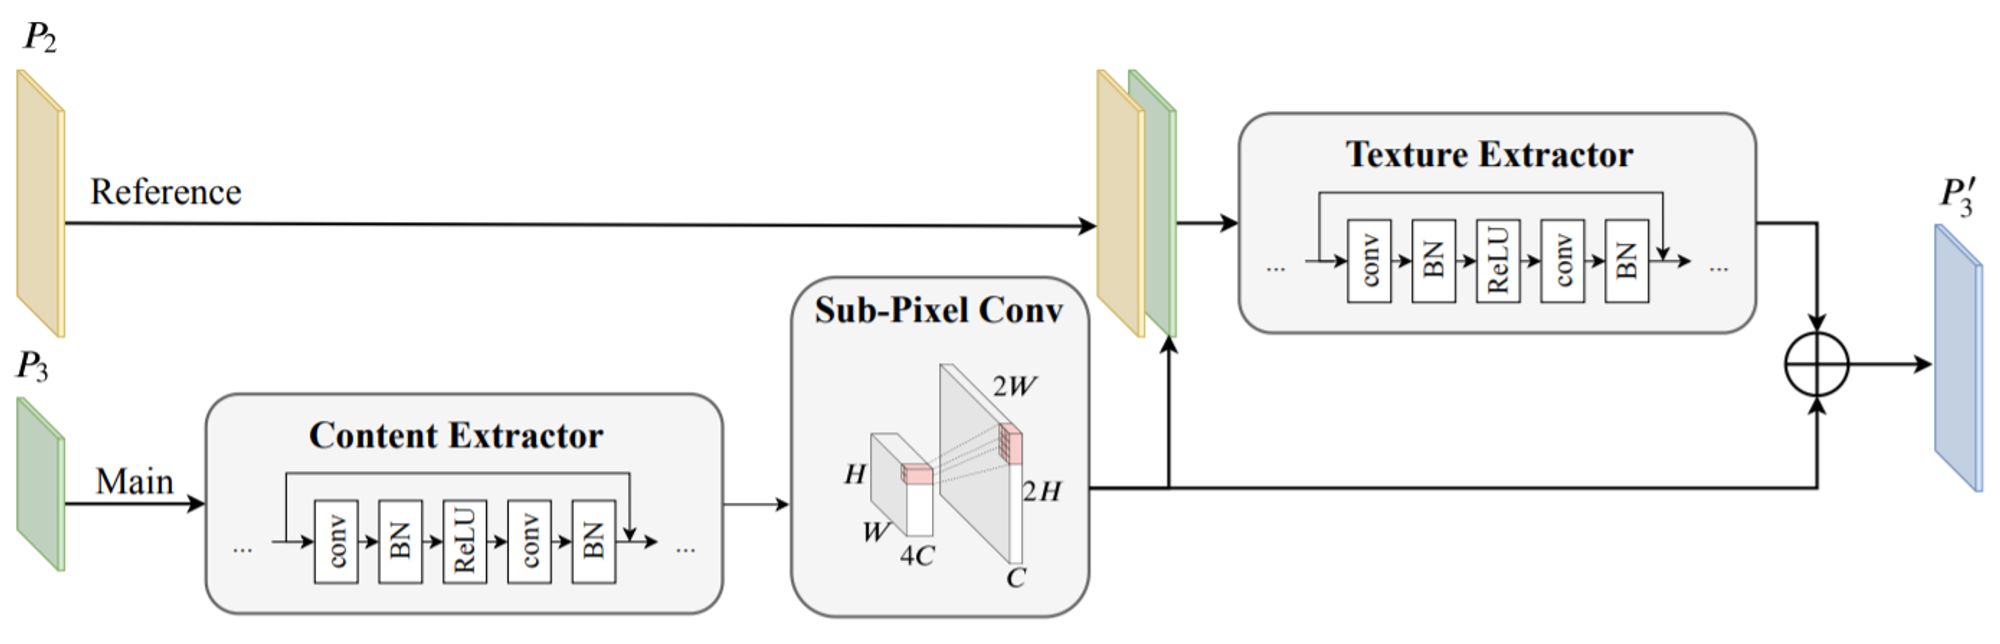
\includegraphics[scale=0.18]{Figures/fft.png}
    \caption{Feature Texture Transfer}
    \label{fig:ftt}
\end{figure}

\newpage
The output $P'_3$ can be defined as:
\[P'_3 = E_t(P_2 \Vert E_c(P_3)_{\uparrow 2}) + E_c(P_3)_{\uparrow 2}\]

,where where $E_t()$ denotes texture extractor component, $E_c()$ denotes content extractor component, $\uparrow 2\times$ here denotes double up-scaling by 
sub-pixel convolution and k denotes feature concatenation. The content extractor and texture extractor are both composed of residual blocks. In the main stream, 
a sub-pixel convolution is applied to upscale spatial resolution of the content features from the main input $P3$ considering its efficiency.
Sub-pixel convolution augments pixels on the dimensions of width and height via diverting pixels on the dimension of channel.


\subsection{Masked-Attention Mask Transformer} \label{mamt}

Mask classification architectures group pixels into N segments by predicting N binary masks, along with N corresponding category labels. 
Mask classification is general enough to address any segmentation or object detection task by assigning different semantics.
However, the  challenge is to find good representations for each segment. Inspired by DETR [], each segment in an image can be represented as a 
C-dimensional feature vector know as object query and can be processed by a Transformer decoder, trained with a set prediction objective. A simple meta 
architecture would consist of three components. 

A backbone that extracts low resolution features from an image. A pixel decoder that gradually up-samples low-resolution features from the output of the 
backbone to generate high-resolution per-pixel embeddings. And finally a Transformer decoder that operates on image features to process object queries. 
The final binary mask predictions are decoded from per-pixel embeddings with object queries. One successful instantiation of such a meta architecture is 
MaskFormer [].


Mask2Former adopts this kind meta architecture, with the proposed Transformer decoder in the Figure \ref{fig:mamt} replacing the standard one. The key 
components of the Transformer decoder include a masked attention operator, which extracts localized features by constraining cross attention to within the 
foreground region of the predicted mask for each query, instead of attending to the full feature map. 

\begin{figure}[h!]
    \centering
    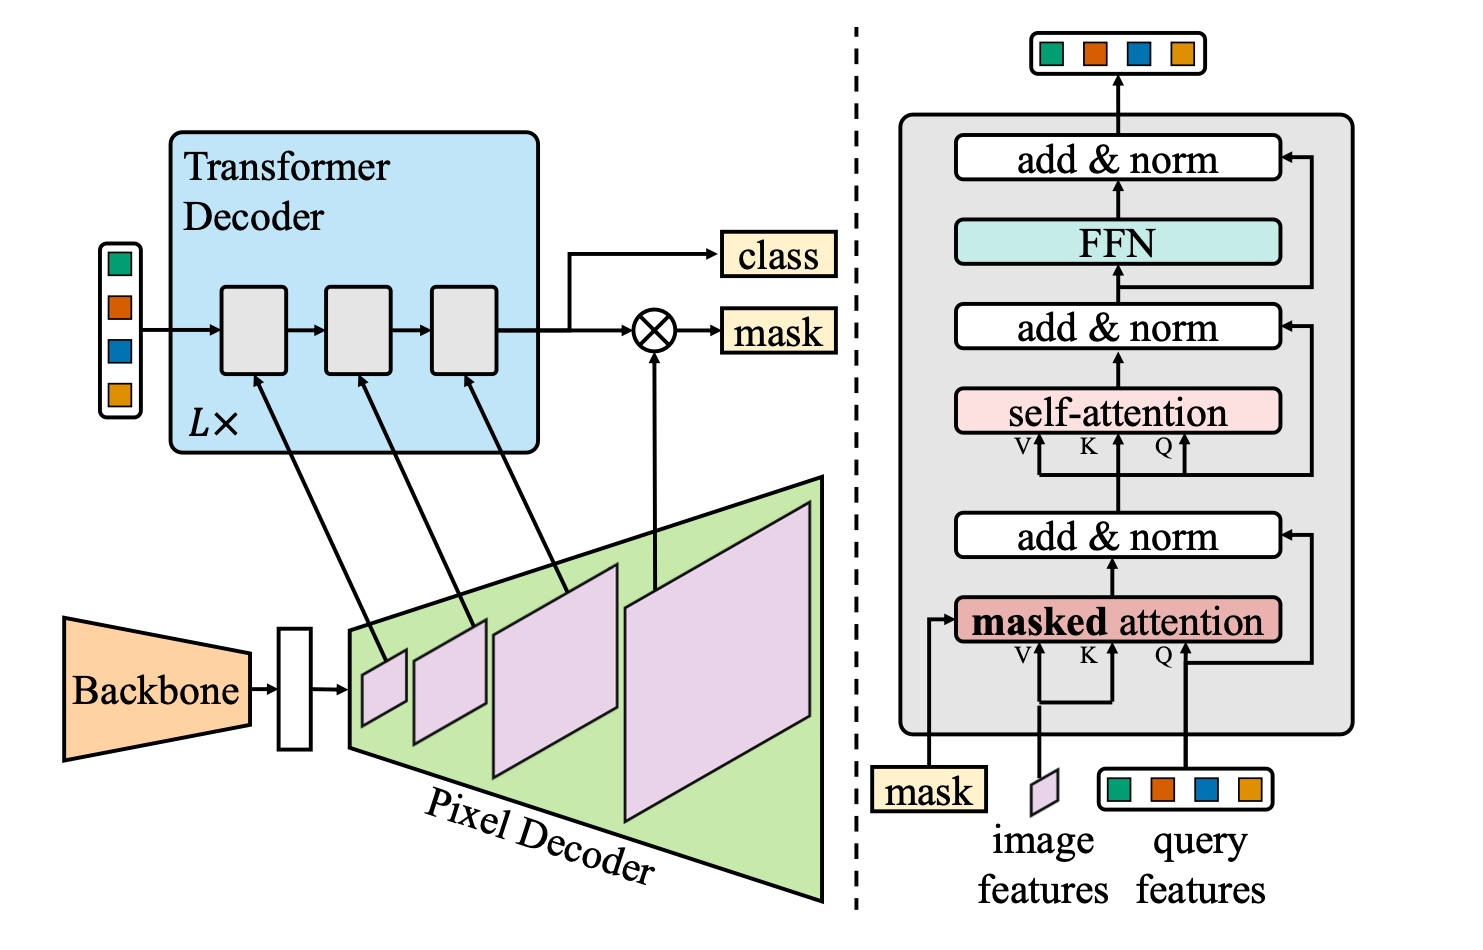
\includegraphics[scale=0.8]{Figures/MaskAttentionMaskTransformer.jpg}
    \caption{Masked-Attention Mask Transformer}
    \label{fig:mamt}
\end{figure}


\newpage
To handle small objects, an efficient multi-scale strategy is proposed to utilize high-resolution features. It feeds successive feature maps from the 
pixel decoder’s feature pyramid into successive Transformer  decoder layers in a round robin fashion. 
Context features have been shown to be important for image segmentation. However, recent studies [] suggest that the slow convergence of 
Transformer-based models is due to global context in the cross-attention layer, as it takes many training epochs for cross-attention to learn to attend to 
localized object regions. 

There is the hypothesize that local features are enough to update query features and context information can be gathered through self-attention. 
For this a masked attention was proposed, a variant of cross attention that only attends within the foreground region of the predicted mask for each query. 
Standard cross-attention computes:

\[X_l = \text{softmax}(Q_l K_l^T) V_l + X_{l-1}\]

Here, $l$ is the layer index, $X_l \epsilon R^{N \times C}$ refers to N C-dimensional query features at the $l$th layer and 
$Q_l = f_Q(X_l-1) \epsilon R^{N \times C} $. Here $X_0$ denotes input query features to the Transformer decoder. $K_l, V_l \epsilon R^{H_l W_l \times C}$ are the 
image features under transformation $f_K()$ and $f_{V}()$ respectively, and $H_l$ and $W_l$ are the spatial resolution of image features, $f_Q$, $f_K$ and $f_V$ are 
linear transformations


Our masked attention modulates the attention matrix via
\[X_l = \text{softmax}(\mathcal{M}_{l-1} + Q_l K_l^T) V_l + X_{l-1}\]

Moreover, the attention mask $M_{l-1}$ at feature location (x, y) is:
\[
    \mathcal{M}_{l-1}(x, y) = 
    \begin{cases} 
    0 & \text{if } \mathcal{M}_{l-1}(x, y) = 1 \\
    -\infty & \text{otherwise} 
    \end{cases}    
\]

Here, $M_{l-1} \epsilon \{0, 1\}^{N \times H_l W_l}$  is the binarized output, thresholded at 0.5 of the resized mask prediction of the previous $(l - 1)$-th 
Transformer decoder layer. It is resized to the same resolution of $K_l$. $M_0$ is the binary mask prediction obtained from $X_0$, before feeding query features
into the Transformer decoder.

High-resolution features improve model performance, especially for small objects [], however, this is computationally demanding. 
Thus the solution being an efficient multi-scale strategy to introduce high-resolution features while controlling the increase in computation. 
Instead of always using the high-resolution feature map, a feature pyramid which consists of both low- and high-resolution features is utilized and 
feed one resolution of the  multi-scale feature to one Transformer decoder layer at a time. Specifically, the feature pyramid produced by the 
pixel decoder with resolution $1/32, 1/16$ and $1/8$ of the original image. For each resolution, both a sinusoidal positional embedding 
$e_{pos} \epsilon R^{HlWl×C}$ and a learnable scale-level embedding $e_{lvl} \epsilon R^{1 \times C}$ is added. 

We use those, from lowest-resolution to highest-resolution for the corresponding Transformer decoder layer as shown in Figure \ref{fig:mamt}. This is 
repeated for a 3-layer Transformer decoder L times. In this case the final Transformer decoder hence has 3L layers. 

More specifically, the first three layers receive a feature map of resolution $H1 = H/32, H2 = H/16, H3 = H/8, W1 = W/32, W2 = W/16, W3 = W/8$, 
where $H$ and $W$ are the original image resolution. This pattern is repeated in a round robin fashion for all following layers.

\newpage
\subsection{Extended Masked-Attention Mask Transformer}

Throughout our extensive research into advanced object detection models and architectures, it became an interesting idea that a hybrid approach would 
yield the most effective results, especially for the task of small object detection. The detailed analysis of various architectures led us to the strategic 
combination of two highly effective models: the Extended Feature Pyramid Network (EFPN) and the Masked-Attention Mask Transformer (MAMT). 
This integration leverages the EFPN’s robust capability in generating precise multi-scale feature maps and initial bounding boxes and masks with great efficiency, 
with the MAMT’s advanced attention mechanisms that refine these masks for superior accuracy that is vital for the Small Object Detection task. 

In this section we are going to analyze our model, the Extended Masked-Attention Mask Transformer or EMAMT starting with the models architecture in the Figure
\ref{fig:emamt}.

\begin{figure}[h!]
    \includegraphics[scale=0.05]{Figures/EMAMT.png}
    \caption{Extended Masked-Attention Mask Transformer}
    \label{fig:emamt}
\end{figure}

Firstly we are going to analyze the EFPN part of the model in the lower left part of the Figure \ref{fig:emamt}, where the EFPN model has as a input,
an image of size $600 \times 600$. The reason for the selection of that size is the backbone we use to generate the rich feature maps for the model.
In our architecture we decided that a pre-trained feature extractor that combines great performance and light design was vital. This combination of characteristics
led us to the choice of EfficientNet [] model and more specifically the EfficientNet-B7 model that uses an input size of $600 \times 600$. Furthermore we decided 
to create five feature maps that have the sizes $(300, 300), (150, 150), (75, 75), (38, 38), (19, 19)$ in order to have a wide range of data for the model to use. 

Alongside the feature maps the EFPN also produces the bounding boxes and the initial binary masks that are going to be used by the MAMT detector. The 
bounding boxes and the masks are implemented on the most detailed feature map $P'2$ that is the result of the addition of the richest spatial map $C'2$ 
and the richest feature map created by the feature texture transfer $P'3$. At the same time we have included a anchor generator model that creates anchors, 
informed based on the mean and standard deviation of the size of the bounding boxes of each dataset in order to conclude the first cycle of detection, between the 
actual data, the anchors and the bounding boxes. In this way we are able to train the EFPN model in parallel to the MAMT model, achieving better convergence.
With the end of the EFPN model we are expecting a set of five  feature maps, a set of bounding boxes and the corresponding classed for each object 
and the initial binary masks. 

The next part of the EMAMT model is the patch and positional embedding we use in order to add to the model the  sense of spatial arrangement among the input 
image patches. Since transformers inherently lack any mechanism to recognize order or position, positional embeddings are crucial for providing this spatial 
context. The creation of the positional embeddings follows the exact same idea as the original paper of MAMT, since it was the implementation of the
sinusoidal positional embedding for images, adapted from the concept originally used in the transformer architecture for natural language processing.
This type of embedding generates position encodings based on sine and cosine functions of different frequencies.


At this point we have a set of five embeddings of the feature maps, a set of bounding boxes and the corresponding classes and the binary masks. Along all
that information the detector of this model we use a set number of queries that in this case is set to $100$, because we wanted to focus on reliable 
detecting a sensible number of objects. For images that contain more than $100$ objects and the annotations we decided to only use the first $100$ of them 
to train the model. Provided all of this data the Vision Transformer architecture can be seen in the Figure \ref{fig:emamt-trm}.

\begin{figure}[h!]
    \centering
    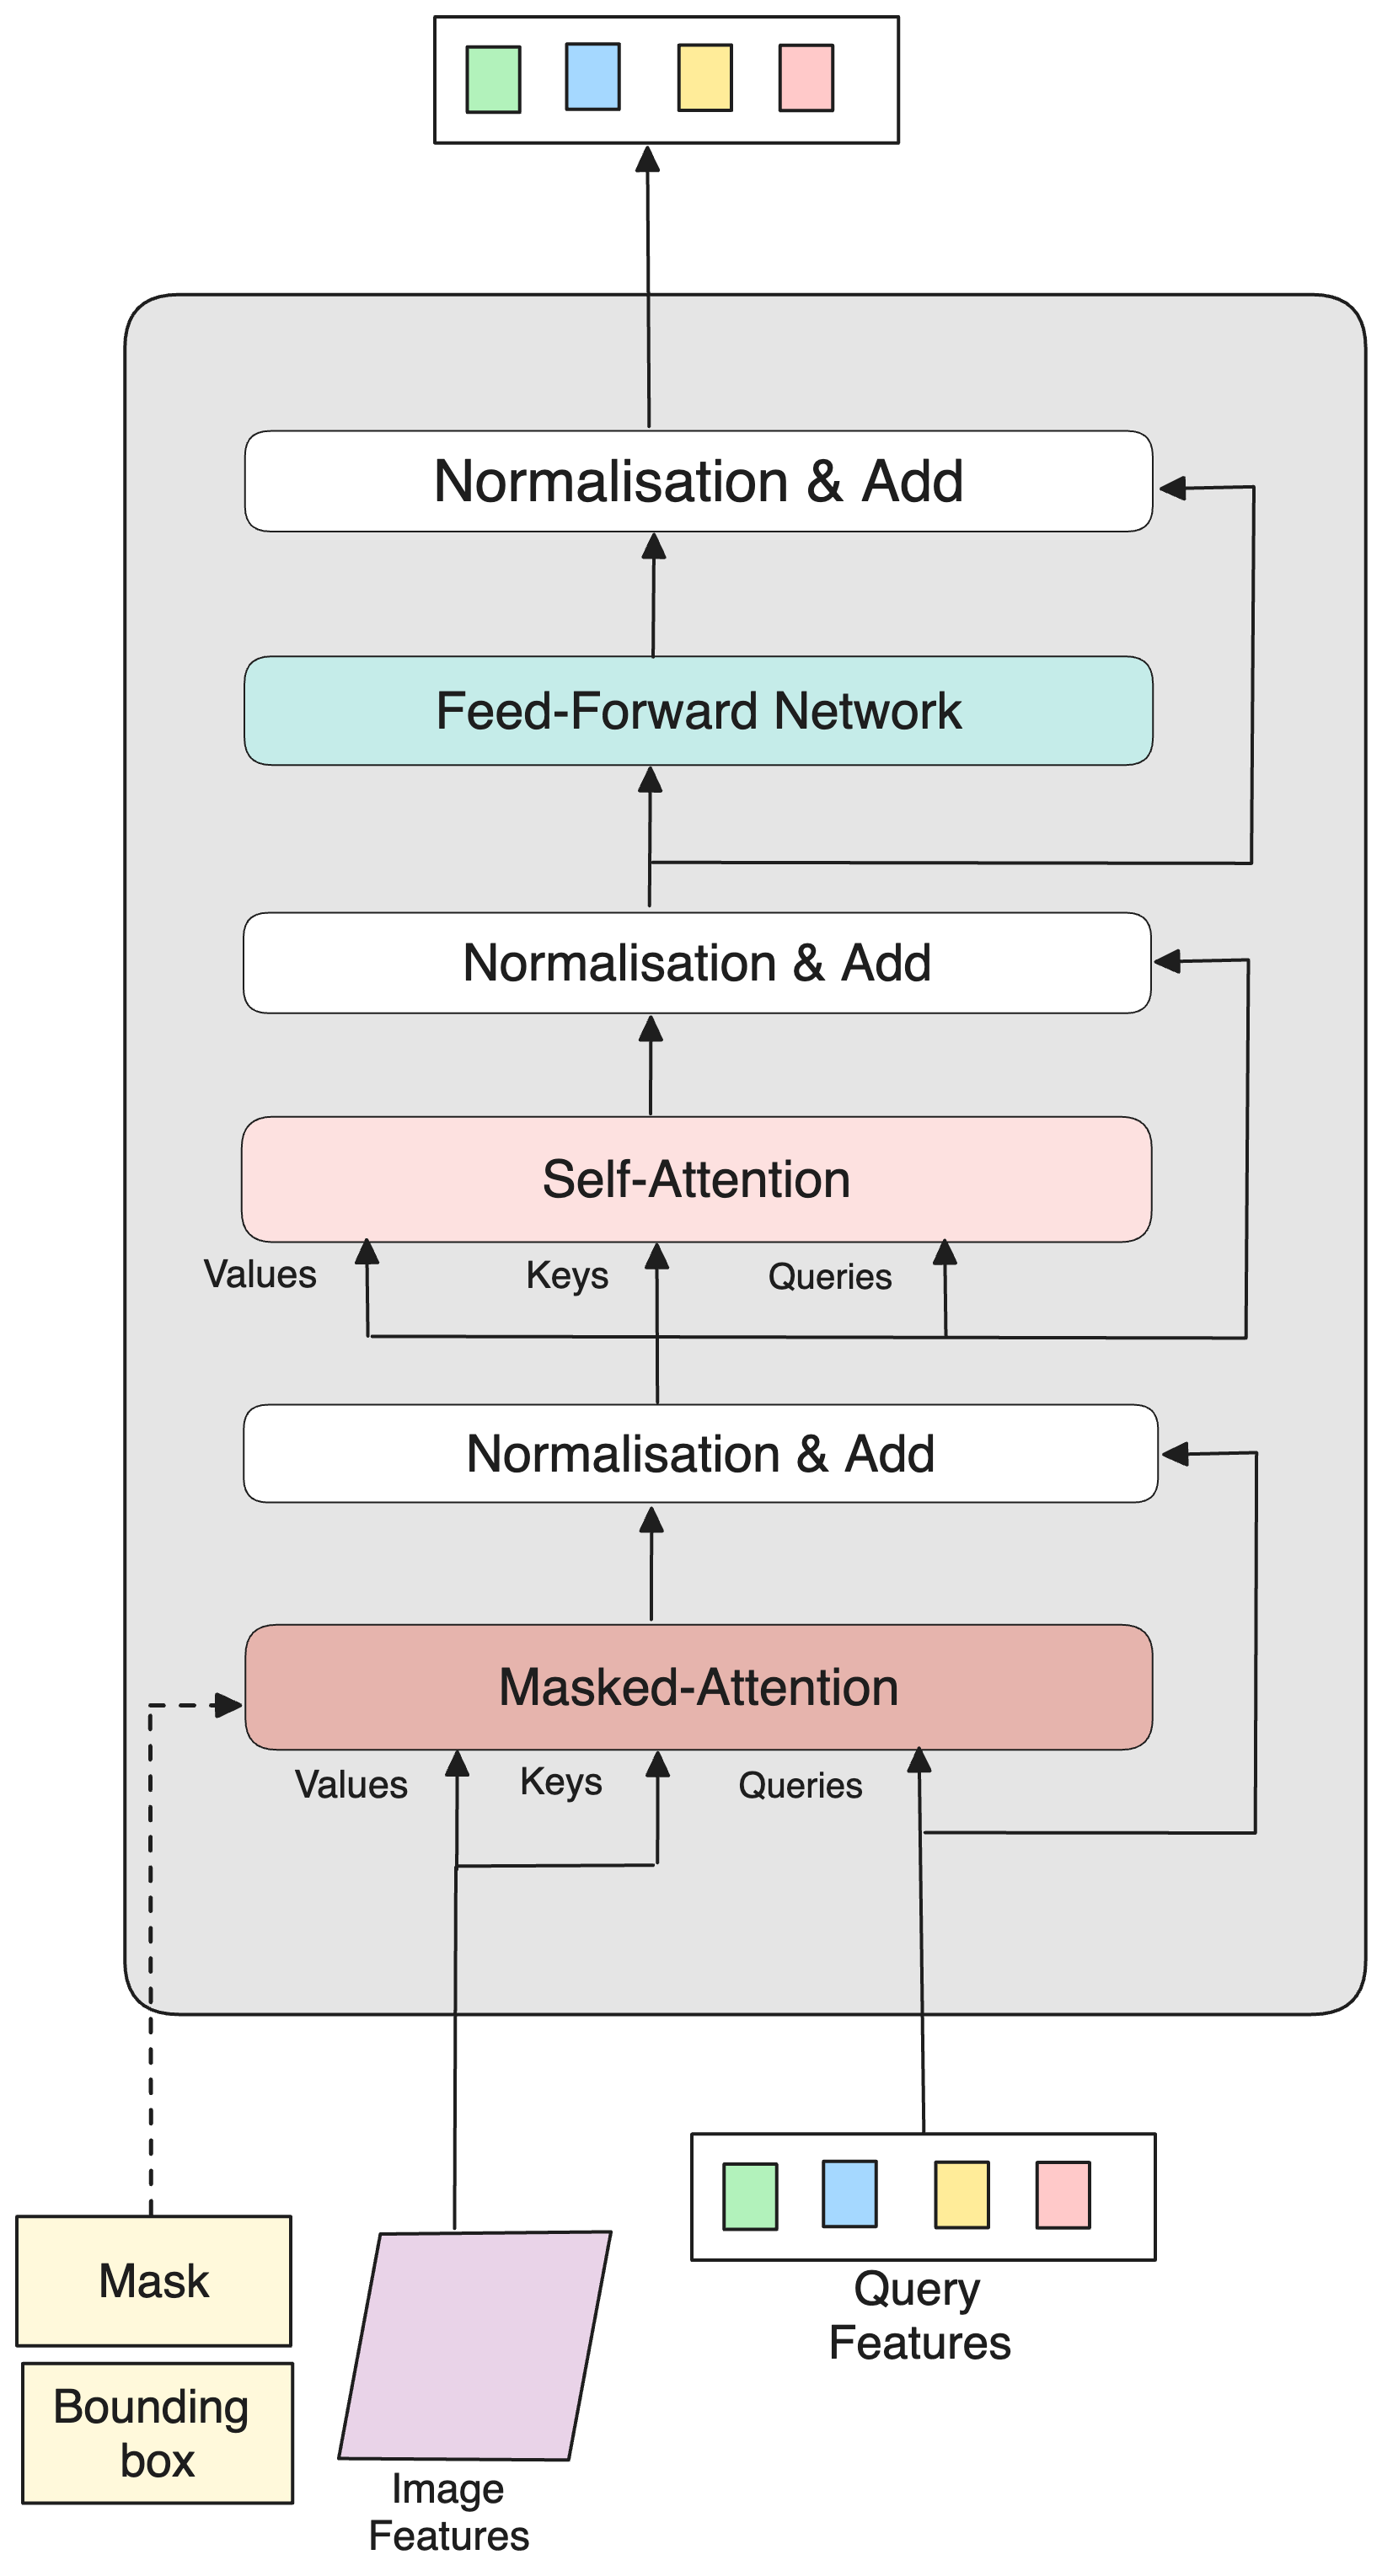
\includegraphics[scale=0.1]{Figures/emamt-encoder.png}
    \caption{Extended Masked-Attention Mask Transformer - Transformer Module}
    \label{fig:emamt-trm}
\end{figure}

\newpage
As mentioned in the section \ref{mamt} we have the hypothesis that local features are enough to update query features and context information can be 
gathered through self-attention. For this reason we use masked attention, a variant of cross-attention that only attends within the foreground region of 
the predicted mask for each query with the aim of better performance and faster convergence. More specifically the masked attention layer is used to focus 
the model’s attention selectively based on certain predefined or learned criteria like the object queries, typically aligning with relevant areas of the 
input image. For instance, in tasks like image segmentation, the masked attention layer might concentrate processing on areas within a specific region of 
interest (ROI), such as the foreground of an image versus the background. This selective attention helps the model to efficiently process only the most 
informative parts of the image, thereby optimizing computational cost.


Following the masked attention, the cross-attention layer has to integrate additional context or features from another source into the transformer’s workflow. 
When placed after a masked attention layer, the cross-attention layer can leverage the focused localized features processed by the masked attention and enrich 
these features with further contextual or supplementary data. 

Lastly after the attention mechanisms—both masked and cross-attention—the FFN acts as a point of non-linear transformation that further processes the refined, 
attention-focused features. This structure allows the FFN to introduce additional complexity and abstraction capabilities into the feature representations.


In order to maximize the capabilities of this model we had to create a custom loss function that takes into consideration all the data created by the model. 
The loss function for the Extended Mask2Former model is designed to jointly optimize object detection and instance segmentation tasks by integrating multiple 
loss components. The total loss \( L_{\text{total}} \) is computed as a weighted sum of the mask loss, bounding box regression loss, and classification loss:

\[
L_{\text{total}} = \lambda_{\text{mask}} \, L_{\text{mask}} + \lambda_{\text{bbox}} \, L_{\text{bbox}} + \lambda_{\text{class}} \, L_{\text{class}}
\]

where:

\( \lambda_{\text{mask}} \), \( \lambda_{\text{bbox}} \), and \( \lambda_{\text{class}} \) are weighting coefficients for each loss component.

\vspace{1.5cm}

\begin{enumerate}
    \item \textbf{Mask Loss}: (\( L_{\text{mask}} \))
    The mask loss measures the discrepancy between the predicted masks \( \hat{M} \) and the ground truth masks \( M \). It uses the Binary Cross-Entropy Loss with logits:
    \[
    L_{\text{mask}} = \frac{1}{N} \sum_{i=1}^{N} \text{BCEWithLogits}\left( \hat{M}_i, \, M_i \right)
    \]

    - \( N \) is the number of matched instances. \\
    - The matching between predicted and ground truth masks is performed using the Hungarian algorithm based on a combined cost of mask Intersection over Union (IoU) 
    and classification cost.
    \newpage

    \item \textbf{Matching via Hungarian Algorithm}

    To align predicted instances with ground truth instances, the Hungarian algorithm solves an assignment problem using a combined cost matrix \( \mathbf{C} \):
    
    \[
    \mathbf{C} = \alpha \left( 1 - \text{IoU}\left( \hat{M}, \, M \right) \right) + \beta \left( -\log\left( \text{Softmax}\left( \hat{C}_{\text{mask}} \right) + \epsilon \right) \right)
    \]
    
    - \( \alpha \) and \( \beta \) are weighting coefficients for the IoU and classification cost components, respectively. \\ 
    - \( \text{IoU}\left( \hat{M}, \, M \right) \) computes the Intersection over Union between predicted and ground truth masks. \\
    - The negative log-likelihood term penalizes incorrect class predictions. \\
    - \( \epsilon \) is a small constant added to avoid taking the logarithm of zero. \\

    \item \textbf{Bounding Box Regression Loss}: (\( L_{\text{bbox}} \))

    This loss quantifies the error between the predicted bounding boxes \( \hat{B} \) and the regression targets \( B^* \) (encoded ground truth boxes relative to anchor boxes \( A \)) using the Smooth L1 Loss:
    
    \[
    L_{\text{bbox}} = \frac{1}{K} \sum_{j=1}^{K} \text{SmoothL1}\left( \hat{B}_j, \, B^*_j \right)
    \]
    
    - \( K \) is the number of anchor boxes. \\ 
    - The regression targets \( B^* \) are obtained by encoding the matched ground truth boxes \( B \) with respect to the anchors \( A \):
    
      \[
      B^* = \text{encode}\left( B, \, A \right)
      \]
    
    - Anchors are matched to ground truth boxes using an IoU-based matching strategy.

    \item \textbf{Classification Loss}: (\( L_{\text{class}} \))

    The classification loss evaluates the discrepancy between the combined class predictions \( \hat{C} \) and the ground truth class labels \( C \). 
    The predictions from both the bounding box branch \( \hat{C}_{\text{bbox}} \) and the mask branch \( \hat{C}_{\text{mask}} \) are combined by 
    taking the element-wise maximum of their softmax probabilities:
    
    \[
    \hat{C} = \max\left( \text{Softmax}\left( \hat{C}_{\text{bbox}} \right), \, \text{Softmax}\left( \hat{C}_{\text{mask}} \right) \right)
    \]
    
    The classification loss is then computed using the Cross-Entropy Loss:
    
    \[
    L_{\text{class}} = \frac{1}{N} \sum_{i=1}^{N} \text{CrossEntropy}\left( \hat{C}_i, \, C_i \right)
    \]
    
    - \( N \) is the number of instances. \\
    - \( C_i \) is the ground truth class label for instance \( i \).
\end{enumerate}
















\newpage

The table below, sorted by the number of parameters, provides a comparative look at various popular object detection models that we have presented in the 
section above. This table highlights models ranging from YOLOv3, known for its balance of speed and accuracy, to more complex architectures like Mask R-CNN, 
which provides high precision at the cost of increased computational resources. Notably, the Extended Masked-Attention Mask Transformer shows how recent 
advancements aim to reduce parameter counts while potentially enhancing model capabilities. This spectrum illustrates the trade-offs between model complexity 
and operational efficiency, guiding decisions in model selection based on specific application needs.

\begin{table}[h]
    \centering
    \begin{tabular}{|c|c|}
    \hline
    \textbf{Model}                                 & \textbf{Number of Parameters (millions)} \\ \hline
    YOLO (You Only Look Once)                      & 62                                      \\ \hline
    Extended Masked-Attention Mask Transformer     & 76.6                                    \\ \hline
    Single Shot    Multibox Detector (SSD)         & Typically around 100                    \\ \hline
    Fast R-CNN                                     & Typically around 150                    \\ \hline
    Faster R-CNN                                   & Typically around 200                    \\ \hline
    FPN with Basic Detector                        & Typically around 200                    \\ \hline
    Mask R-CNN                                     & Typically around 250                    \\ \hline
    R-CNN                                          & Varies, typically less than 250         \\ \hline
    \end{tabular}
    \caption{Comparison of Object Detection Models Sorted by Number of Parameters}
    \label{tab:model_parameters}
    \end{table}
    
